\documentclass[bsc,frontabs,twoside,singlespacing,parskip,deptreport]{infthesis}     % for BSc, BEng etc.
\usepackage{graphicx} %package to manage images
\graphicspath{ {images/} }

\usepackage[utf8]{inputenc}
\usepackage[TS1,T1]{fontenc}
\usepackage{fourier}
\usepackage{array, booktabs}
\usepackage[x11names]{xcolor}
\usepackage{colortbl}
\DeclareCaptionFont{blue}{\color{LightSteelBlue3}}

\newcommand{\foo}{\color{LightSteelBlue3}\makebox[0pt]{\textbullet}\hskip-0.5pt\vrule
  width 1pt\hspace{\labelsep}}

\begin{document}

\title{StarCraft Brood War as an Agent Learning Platform Interim Report}

\author{Nantas Nardelli}

\course{Artificial Intelligence and Computer Science}
\project{4th Year Project Report}

\date{\today}

\abstract{

  In the past couple of years the field of Reinforcement Learning has been
  shaken up by what is now labelled as Deep Reinforcement Learning, that is the
  process of using deep architectures such as convolutional neural networks to
  approximate some of the functions required in a reinforcement learning
  process. The shift of part of the community to this particular methodology
  appears to have created the need for test-beds that are unusually more
  data-hungry, data-driven and related to vision or natural language processing.
  Moreover, the inherent hierarchy of those approximation techniques calls for
  advances in Hierarchical Reinforcement Learning. To satisfy these needs we
  have developed a platform for agent learning based on a classic
  Real-Time-Strategy (RTS) game, Starcraft Brood War, and we have built an
  interface to be able to perform experiments based on a popular Deep Learning
  framework, Torch. To test the framework we have then ported the recent
  ``deep'' variant of Q-learning, DQN and made it train on a few simple maps.
  Finally we have started developing an Hierarchical Reinforcement Learning
  algorithm for primitives discovery.
}

\maketitle

% \section*{Acknowledgements}
% Acknowledgements go here.

\tableofcontents

%\pagenumbering{arabic}


\chapter{Introduction}

Addressing the problem of Artificial Intelligence is very interesting but
extremely difficult, as intelligence must not only be developed, but also tested
adequately before it is possible to fully classify it appropriately.
Reinforcement Learning (RL) provides a view on intelligent behaviour that stands
on the shoulders of lots of research in fields such as neuroscience, psychology
and mathematics, and whose formalisation is mostly agreed upon in the AI
research community\cite{Sutton:1998:IRL:551283}. Reinforcement learning is used
to describe the process of learning to control the environment optimally, but
this process is not very scalable for environments that approach a level of
complexity similar to the real-world, as the agent must sufficiently solve the
problem of both creating a useful representation of sensory inputs and
generalise over it for long term learning. To tackle the representation problem
the community lately started emphasising the usage of a deeper approach to
machine learning, deep learning, where efficient, scalable and high-capacity
models can learn some form of distributed representation of their
input\cite{lecun2015deep}.

\section{Games as virtual learning environments}

Through the decades several benchmark suites have been developed to allow the
reinforcement learning and AI community to build and test their algorithm in a
scientific fashion. These were usually in the form of either pure decision
problems such as the multi-armed bandit problem[CITE HERE] or interactive and
environmentally rich scenarios such as gridworld. Part of the community also
went on focusing on using robotic competitions to advance the state of the art
of reinforcement learning algorithms[PETER STONE CITE HERE], while some other
preferred remaining within the boundaries of software and use simulation
environments to carry on their research[CITE CITE CITE]. Finally with the years
the use of computer games as AI benchmark also has also become common, with new
comprehensive gaming suites such as the Atari Learning Environment (ALE)[CITE
ALE HERE] and open source ports of popular games like Warcraft[STRATAGUS HERE].

\section{Deep Reinforcement Learning}

The usage of deep learning models such as Convolutional Neural Networks to
approximate and represent part of the functions required for a reinforcement
learning process to work and learn was coined Deep Reinforcement Learning in
2013 and has since become a popular solution to some of the complex
representation problems in many RL scenarios\cite{mnih2013playing}.

\section{StarCraft Brood War}
Real time strategy (RTS) games have historically been a source of complex
problems for AI researchers. The domain they represent is essentially a
simplified military simulation where players fight live and fight in a
fixed-size 2D map for the control of the resources lying all over the map to
build armies and an economy that allows them to win battles and finally the
overall game. The variety of AI and decision problems that this typology of
games involves and requires solving include (but are not limited to):

\begin{itemize}
  \item Decision making under uncertainty
  \item Opponent modelling and Learning
  \item Resource management
  \item Real-time planning
  \item Exploration/exploitation dilemma
\end{itemize}

Those are all terribly challenging problems that have spawned several techniques
and even entire fields of research. The creation of a machine learning system
that can at least partially solve all those problems and therefore have the
chance to be able to play with a human opponent is far from being close, even
with the relatively game-changing performances of Deep Reinforcement Learning.

In the past years several RTS research platforms have emerged, the most
prominent ones being Stratagus, OpenRTS and Wargus, however the lack of polish,
missing game mechanics and features that are normally available in commercial
RTS games, and lack of community does not make them ideal to do AI research,
especially now that some important parts of it rely also on good amounts of
available data to be fruitful. A more feasible solution was instead to take one
of the popular commercial games and adapt it as to make it an AI testing suite;
in our case, we chose StarCraft.

Starcraft is a relatively old commercial game that represents the quintessence
of Real Time Strategy (RTS) games. Its code is unfortunately completely closed
and Blizzard have never really opened the game to modifications. However a few
users have developed an interface to read the memory of the game and modify it,
called Brood War Application Programming Interface (BWAPI).

\section{BWAPI}

BWAPI is a C++ API that allows to interact with StarCraft and StarCraft Brood
War. It allows to create agents by controlling directly the entire client or by
using DLL injection to dynamically run the AI code within the address space of
the game. This interface has become somewhat popular within the community and
around it have spawned a couple of tournaments and tens of developers willing to
help with its maintenance. For our purpose we had to add some functionality to
the API to allow it to be usable as a (deep) reinforcement learning environment.

\chapter{The Project}

\section{Architecture}

\begin{figure}[h]
    \centering
    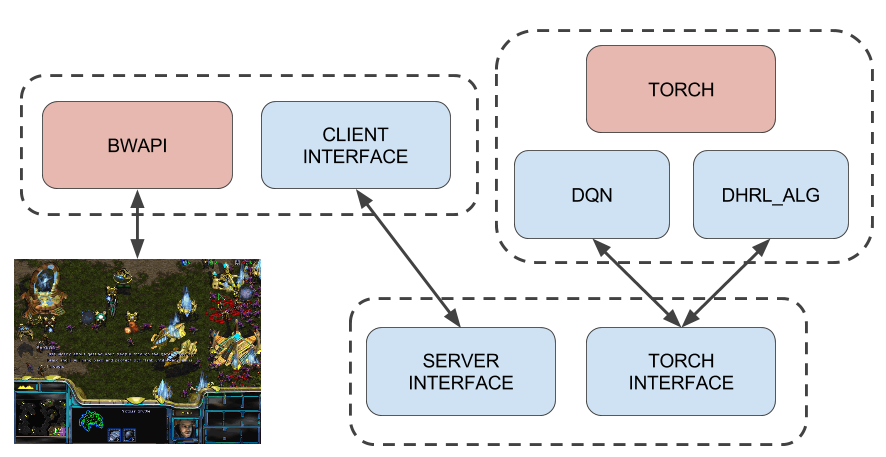
\includegraphics[width=\textwidth]{architecture}
    \caption{The project's current architecture}
    \label{fig:arch}
\end{figure}

Our entire architecture looks like the one in Figure \ref{fig:arch}: a C++
client initialises BWAPI and communicates through shared memory with a running
instance of StarCraft Brood War; the client is then linked to a server also
written in C++ running on a Linux machine through a blocking socket connection,
which initialises luajit, Torch, the CUDA environment and then runs the AI.

The client not only manages the game and parses its information, but it also
takes advantage of the standard Windows API to access the graphical output
generated by the game and extract it as a standard integer array, so that it can
then sent to the server and used as the input state for our algorithms together
with the game state. After several optimisation this operation doesn't take a
significant toll on the overall performances, but a text-based configuration
system has also been included to active features such as this one. The game
information is instead collected using BWAPI and then encoded in a Google
ProtoBuffer, a standard serialisation object that encodes arbitrary data
structures into byte arrays and that is fast and that allows to check for data
presence and validity.

As we previously mentioned, BWAPI allows to do DLL injection and place the AI
binary code directly into the StarCraft process. This is the preferred method
used in both at SSCAIT and AIIDE, but it doesn't give a good amount of control
on the game itself, and makes it therefore difficult to prepare good
experimental settings. Since those two methods are exclusive, we decided to use
the other client-server based interface. The idea was to simulate most of the
ALE interface to allow for easy interoperability with DeepMind's DQN codebase
and other codebases based on that particular one, and the closest model was the
one that was most decoupled from the game.

\section{C++ server to Torch: luajit interface}

After the game state and the image messages get passed through socket connection
to the linux server, those need to be passed to the lua process so that it can
own them and use them appropriately. To do so we wrapped the entire C++ server
interface in lua objects by creating a dynamic library and loading it into lua
using the LuaJIT.

LuaJIT is a Just-In-Time compiler for Lua, which allows to connect high
performance C and C++ code with the more high level Lua scripting language,
therefore simplifying the process of writing high-level interfaces while
maintaining the speed of faster but lower-level languages. There are a few ways
for this process to happen, but we essentially decided to directly load the
compiled binary with the C++ object definitions and declarations into the lua
ecosystem via an LuaJIT internal declaration and linking system. The objects are
then wrapped with the Torch class interface[CITE HERE], which then can be used
completely.

Translating the image was a slightly more difficult process, because the format
Windows uses to store bitmaps is largely unsupported one in the Linux ecosystem.
The conversion to the format used by Torch was optimised by noticing that the
colour channels are completely separate and that some pointer math is enough to
essentially allow us to use a threaded parallel loop and speed up the copying.
We tried also acting on the stride information used by the Tensor classes in
Torch, but it made other operations very slow (all the ones that actually
modified the tensor itself), because the assumption of continuous data array
could not hold anymore.

\section{Filtering the game state}

Because of its nature as an RTS, it's not easy to extract the totality of the
information that StarCraft produces within a game. In particular, it's not clear
in what ways a programmer should explore the state and which objects and
relations should be explicitly mapped. For instance, we can spatial information
about units and buildings, but collecting information about all the technologies
that each building can produce would mean iterating through all the possible
game objects, checking their existence and creating a huge information tree,
most of which is not necessarily useful to a reinforcement learning system. To
solve this issue we decide to limit our experiments to a few unit classes and to
give access to our models only to their positions and health, without caring
about upgrades or other skills. The set of unit classes includes only Terran and
Zerg units, and are workers (of any kind), soldiers (marines), healers (medics)
and buildings. Because we are not sending information about building usage, we
only need to provide their position and life points.

\section{Interfacing with DeepMind's DQN}

Once the interface was complete and most of the bugs were ironed out, we
proceeded to learn and adapt the code from DeepMind's Nature paper to work with
our project interface. Ultimately we made our interface look exactly like ALE's,
so that very few edits were needed to be made to their codebase. However, a lot
of code related to the different ATARI games was stripped and the configuration
layer was in general simplified.

Unsurprisingly, we discovered with a few preliminary tests that standard DQN was
simply not able to solve most of our maps. In particular, two big issues need to
be addressed for standard deep Q-learning to successfully complete even some
basic part of the game.

\subsection{Starcraft is inherently hierarchical}

As with all RTSs, the game forces players to focus on building solid overall
long-term game strategies and local short-term focused tactics completely in
parallel, often with the clear objective of making the player choose certain
tradeoffs that will benefit long versus short term goals. As a strategy game, we
can therefore see that policies are structured and hierarchical, because certain
strategy might spawn certain tactics with parameters entirely dependent on the
``super-policy''. Additionally Starcraft is also hierarchical in its state and
value, because of the existence of classes available only after certain inter
objectives have been reached, or even just because of the dependency on the
skill tree to develop both militarily and economically.

\subsection{Visual information are completely policy dependent}

As previously mentioned, with most of the roms used within ALE the visual data
contains the full state of the game. That is, assuming we have a good
understanding of the score function, the image given by ALE essentially gives us
all the information we need to get well the most useful action at any given time
with reasonable results. In Starcraft the visual feedback purely represents the
state of the game at a specific point in the map - point usually chosen by the
player through keyboard or mouse actions - and unless the user puts time and
effort in dynamically exploring the map to update his world knowledge an idea of
the general state of the game can only be looked up by observing the extremely
compressed minimap (Figure \ref{fig:one_star}).

\begin{figure}[h]
    \centering
    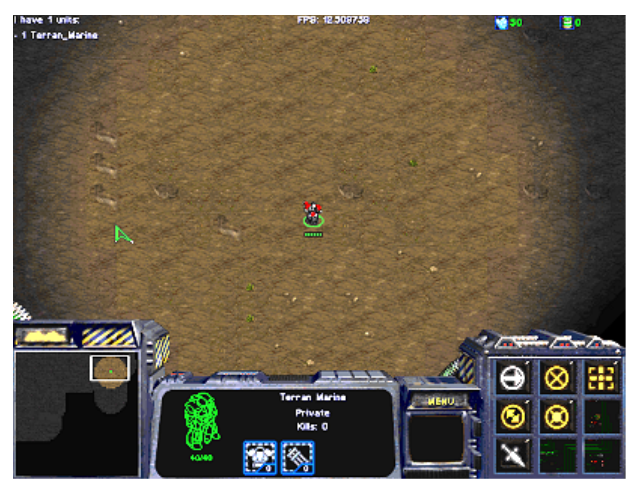
\includegraphics[width=\textwidth]{star_one}
    \caption{The project's architecture}
    \label{fig:one_star}
\end{figure}

Additionally the minimap is also affected by the so-called Fog of War, a feature
in most RTS games that prevents players from observing the state of locally
explored but unobserved zones at a specific time. This means that to fully win
the game the player is forced to continuously explore the state of the game,
regardless of whether they have a more or less complete notion of the topology
of the map. In reality, Starcraft allows us to cheat and disable the Fog of War,
making exploration a one-shot process i.e. once the map is explored it’ll be
“observable” through the entirety of the match.

\begin{figure}[h]
    \centering
    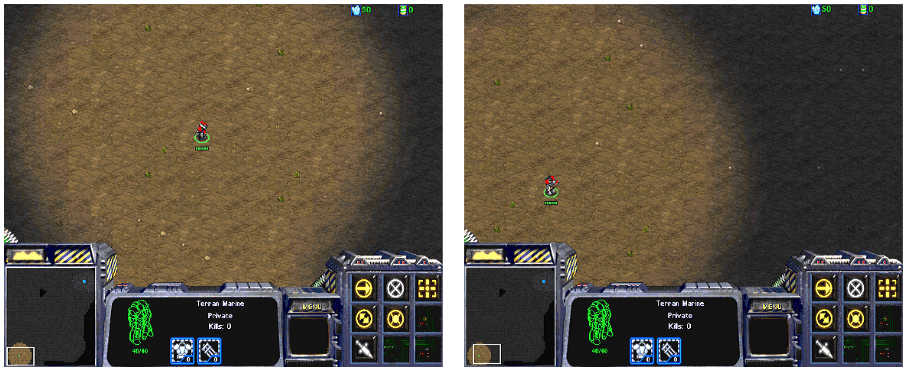
\includegraphics[width=\textwidth]{double_star}
    \caption{The project's architecture}
    \label{fig:double_star}
\end{figure}

Starcraft’s visual feedback by itself (i.e. even without encoded features) is
therefore essentially non-Markovian in how it represents the state of the game.
Starcraft players are required to move the window to gain information, and the
image changes drastically depends on where the window is (Figure
\ref{fig:double_star}), so unless there is some form of memory to collect the game
state, we cannot only use the visual data as input. My conjecture is that
creating an encoded representation of the entire state of game is by itself an
unsolved mixed deep learning (representation) and RL problem, as the variance in
the input is simply too large and it's entirely based on the learnt policy for
both unit actions and screen/environment actions.

\section{Tackling the hierarchical problem}

The issue itself is of policy learning. That is, theoretically we can imagine a
policy that maps all the possible states of the game, with the problem that it
would be clearly become very big even considering two units and the smallest map
size (64 by 64 pixels). When we imagine games with hundreds of units, larger
maps and we add some unit data such as possible actions, life points, energy
points and further information the state quickly explodes and the problem
becomes intractable. To try tackling this from a reinforcement learning
perspective we need to take advantage of the intrinsic hierarchy of actions from
a decision making point of view. To do so, we can use techniques originating
from a the field called Hierarchical Reinforcement Learning.

The idea of splitting the learning process to tackle sub-problems and then
generalise over them has been a source of research for now a few decades.
Several techniques and methodologies have been invented over the years, some of
them trying to decompose the MDPs and act on the decomposed value functions
(MAXQ), some of them using gating structures and learning linker functions, some
of them acting directly in the policy and MDP spaces (Options).

In our case, the simplest way to tackle StarCraft's policy problem is to
iteratively learn about useful sequences of actions, but to do this we need to
``guide'' the agent towards learning the correct primitives and we need to
tackle the simplest possible map, i.e. a map topologically flat in which within
its boundaries agents can move in all directions without constraints, where
there is only one type of enemy and controllable unit and where the only goal is
to maximise the time spent alive.

To learn the primitives we have created a series of random maps with close
boundaries where agents are forced to move mostly in one chosen direction.
Instead of specifically learning a policy, we instead learn the fitness value of
a specific action. Once we have done a few iterations and we know what are the
best actions, we combine them in several ways and we add those new combinations
to the set of possible actions. Doing this process until we stop creating useful
functions should allow us to discover useful primitives with different levels of
complexity.

Once we have learnt those primitives we can then test them with the
aforementioned flat map with additional units and then possibly use additional
models to control the global strategy of the units. The key idea is that we can
keep the same reward system and state representation by doing all this process
for each unit.

\newpage

\section{Final Semester Timeline}

The next steps to complete the project are included in the following table.

\begin{table}[h]
  \begin{center}
    \renewcommand\arraystretch{1.4}\arrayrulecolor{LightSteelBlue3}
    \captionsetup{singlelinecheck=false, font=blue, labelfont=sc, labelsep=quad}
    \caption{Timeline}\vskip -1.5ex
    \begin{tabular}{@{\,}r <{\hskip 2pt} !{\foo} >{\raggedright\arraybackslash}p{\textwidth}}
      \toprule
      \addlinespace[1.5ex]
      22nd January & Addition of infrastructure (no-model) for local primitive discovery. \\
      29th January & Implementation of learning model for local processes. \\
      5th February & Implementation of uniform state-representation and correct reward system. \\
      12th February & Evaluation and experiments on DQN. \\
      26th February & Evaluation and experiments on hierarchical processes. \\
      4th March & Beginning of report drafting process. \\
      11th March & Initial draft of project report. \\
      18th March & More work on project report. \\
      25th March & Final draft of project report. \\
      31st March & Submission of complete project report. \\
    \end{tabular}
  \end{center}
\label{tab:timeline}
\end{table}

% use the following and \cite{} as above if you use BibTeX
% otherwise generate bibtem entries
\bibliographystyle{plain}
\bibliography{thesis}

\end{document}
